\section{Discussion and Conclusions}
\label{sec:conclusions}
\label{sec:comparison}
\emph{In short: the Frequentist and Bayesian analyses give the same $\Araw=-0.044\pm0.009\,(\text{stat})\pm0.007\,(\text{syst})$, $5.2$ standard deviations from zero, with validated intervals; they differ in the meaning of the numbers and of the tests, not in their values.}
On this problem the Frequentist profile-likelihood fit and the Bayesian posterior are equivalent in value, uncertainty and coverage: with a common selection and mass model they give $\Araw=-0.0441\pm0.0085\pm0.0072$ and $-0.0443\pm0.0085\pm0.0070$ (statistical, systematic), a nonzero asymmetry at $5.2$ standard deviations, stable under the thirteen variants (the dominant systematic contribution is the particle-identification requirement) and concentrated in the Dalitz region of the published analysis outside the $\phi(1020)$ ($-0.234\pm0.025$ against $-0.239\pm0.020$).

The numbers coincide, the statements do not. The credible interval states that $A$ lies in $[-0.0528,-0.0358]$ with $68\%$ probability given the data and the prior; the confidence interval $[-0.0526,-0.0356]$ is the set of values that the data do not reject, and its $68\%$ is a property of the procedure that the bootstrap and the toy experiments verified\appref{app:ext_comp}. The Frequentist test of $A=0$, $p=2\times10^{-7}$, is independent of the prior; the Bayes factor, $BF_{10}\approx9\times10^3$, depends on its width (Sec.~\ref{sec:bayes_factor}), and for $A_b=-0.040\pm0.018$ a Frequentist test would call $2.3\sigma$ a hint while $BF_{01}\approx3.5$ mildly favors $A_b=0$. The Frequentist fit adds an unbiased estimator at the minimum variance bound; the Bayesian analysis adds sampling diagnostics and a posterior predictive check. Figure~\ref{fig:checks_profile} shows the profile likelihood and the marginal posterior of $A$ on the same axis.

\begin{figure*}[t]
\centering
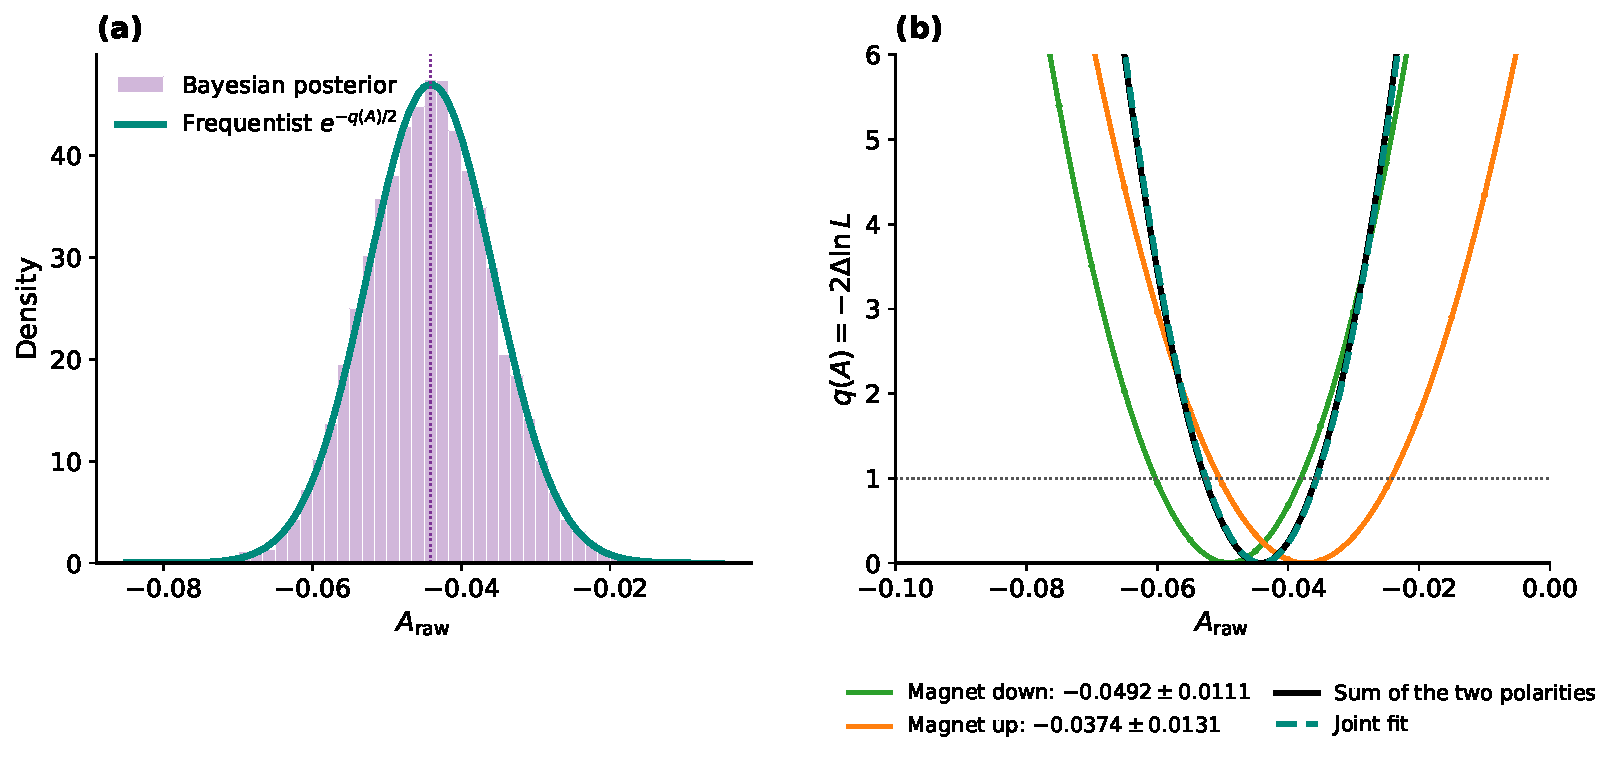
\includegraphics[width=0.95\textwidth]{figures/short_profile_polarity.pdf}
\caption{(a) Frequentist profile likelihood, $\exp[-q(A)/2]$ normalized, and Bayesian marginal posterior of $A$. (b) Profile curves $q(A)$ of the two magnet polarities (parabolic fits to the points), their sum and the joint fit.}
\label{fig:checks_profile}
\end{figure*}

\label{sec:comparison_published}
The published analysis~\cite{lhcb_cpv_2013} finds $-0.060\pm0.007$ on a larger sample with a richer model\appref{app:ext_comp}; with the same $D^0$ veto the Bayesian fit gives $-0.0496\pm0.0088$, within $0.93\sigma$. The raw asymmetry is not the $CP$ asymmetry, $\ACP\approx\Araw-A_P-A_D$ (Eq.~\eqref{eq:acp}): the $5.2\sigma$ here is the significance of a nonzero raw asymmetry, not of $CP$ violation. Three limitations bound the result\appref{sec:limitations}: no tested model reaches $\chi^2/\mathrm{ndof}\approx1$, although $\Araw$ does not depend on the signal shape; no production or detection correction is applied; and the local Dalitz-plane asymmetries are counts without background subtraction. A machine-learning selection leaves $\Araw$ unchanged within its statistical spread\appref{sec:ml}, and the natural next step is a control-channel correction.

\subsection{Additional Results}
\emph{Numerical agreement.} The estimates of the two fits differ by $0.0002$, both uncertainties are $0.0085$, and sideband subtraction gives $-0.0503\pm0.0083$\appref{sec:comparison_numbers}.

\emph{Profile, posterior and polarities.} Profiling and marginalizing the eleven nuisance parameters give the same distribution of $A$, since $A$ is almost uncorrelated with them; the two polarities agree and their combined likelihood reproduces the joint fit; the $68\%$ and $95\%$ regions in $(A,A_b)$ of the profile ($\Delta\mathrm{NLL}$ at $2.30$ and $5.99$) and of the highest posterior density coincide, with $A=0$ outside both\apprefs{sec:checks_profile}{sec:checks_region}.

\emph{Tests and goodness of fit.} The exact binomial test on all candidates gives $6.1\sigma$. The same fit has $p=0.03$ in $2.5\,\MeV$ bins and $p\approx5\times10^{-6}$ in $10\,\MeV$ bins: the $p$-value of the binned $\chi^2$ depends on the binning as much as on the model\appref{app:ext_comp}.

\emph{Low statistics.} Credible and confidence intervals coincide in value and coverage from $\sim2\times10^4$ down to $50$ candidates\appref{sec:bayes_lowstat}.

\emph{Published analysis.} It has $22{,}119\pm164$ signal candidates, a Cruijff signal and misidentified and partially reconstructed backgrounds; its corrections move $-0.060$ to $-0.043\pm0.009\pm0.003\pm0.007$ and cannot be assumed for another selection\appref{app:ext_comp}.

\emph{Machine learning: labels and models.} A classifier separates the signal-enriched window from the sidebands ($15{,}130$ and $1940$ candidates, $20$ features, $60/20/20$ split) and, by the Neyman-Pearson argument of CWoLa, is also the signal/background classifier; the tree ensembles and the neural network reach test AUC $0.857$--$0.864$, $0.09$ above the linear models and indistinguishable within $0.012$, with gradient boosting as reference\apprefs{sec:ml_labels}{sec:ml_models}.

\emph{Machine learning: regularization and uncertainty.} The linear model does not overfit, gradient boosting overfits beyond $\sim150$ stages without losing test AUC, and class weights bias the probabilities, corrected by isotonic recalibration (Brier score $0.122\to0.062$); the mean per-candidate uncertainties are $0.178$ (Random Forest), $0.095$ (MC dropout) and $0.050$ (deep ensemble)\apprefs{sec:ml_regcal}{sec:ml_uncertainty}.

\emph{Machine learning: Dalitz plane and selection.} K-means with $K=8$ finds two clusters beyond $3\sigma$ ($\chi^2=46.4$ for $7$ degrees of freedom), the pattern of the fixed binning ($80.8/31$): negative at low $m^2_{\mathrm{lo}}$, positive at high $m^2_{\mathrm{hi}}$. A cut at $0.5$ on the score keeps $92\%$ of the signal and $36\%$ of the background and gives $-0.0451\pm0.0087$ (Bayesian) and $-0.0447\pm0.0086$ (Frequentist), within the spread of a subsample, with counting too; the hyperparameter search gains at most $0.005$ in AUC (winner's curse), and the selection cannot remove the misidentified background\apprefs{sec:ml_kmeans}{sec:ml_stability}.
